%!TEX root = ../../main.tex
%========================%
\section{大魔神ライブ}
%======================

%----------------------------%
\subsection{サイリウムを奢られる}
%----------------------------%

我々大魔神調査隊はいよいよ大魔神との対決に臨まんと会場の建物入りを果たした。自分が勝手に想像していたライブ会場とはかけ離れたカラオケの受付のようなエントランス。変な椅子を見つけそこそこ楽しかったが、開場まではなんと1時間以上も持て余していた。何か、本番前に用意すべきものは無いか。監督であるアツム氏により「ライブ行くんならサイリウムないとあかんやろ」という助言が与えられた。\\

%----------------------------%
\subsubsection{サイリウム}
%----------------------------%

この項では、サイリウムとは一体どのような光る棒なのかを述べる。\\
一般的にサイリウムと呼ばれている光る棒は以下の写真のようなものであることが多い。

\begin{figure}[H]
\centering
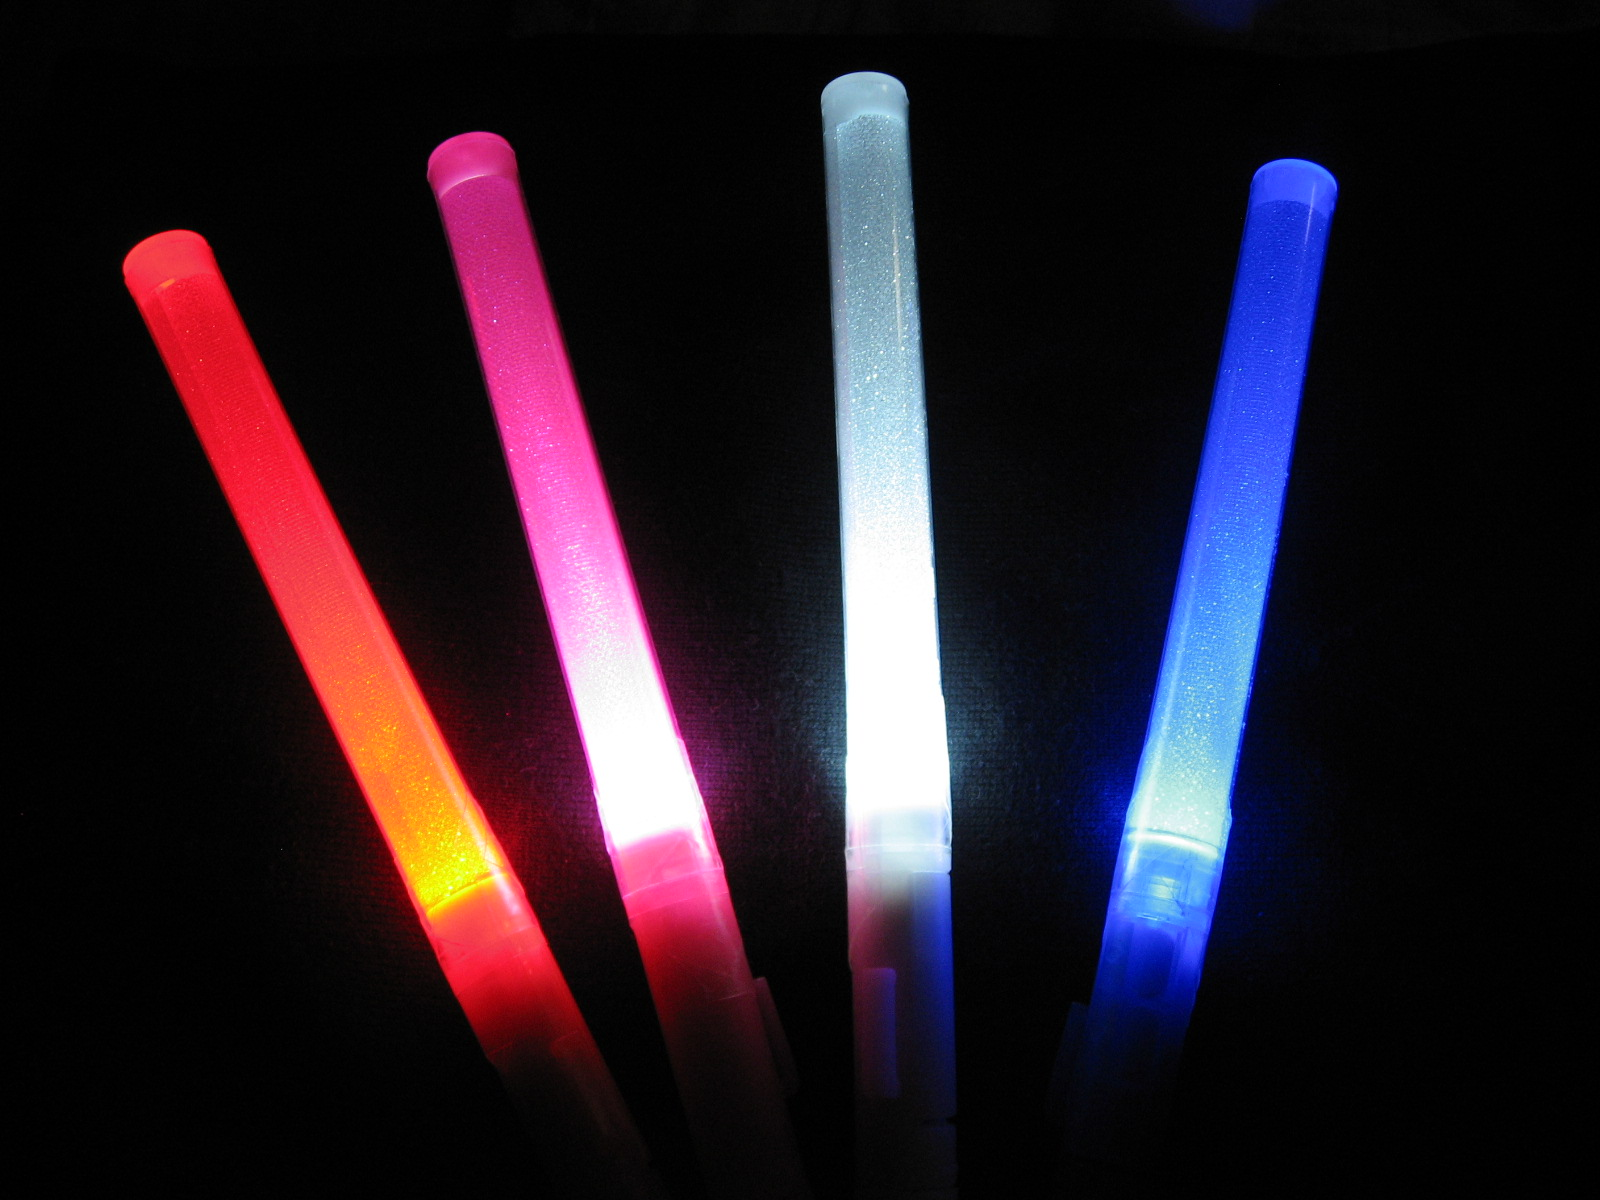
\includegraphics[scale=0.3]{./section/sasakiLIVE/figures/penlight.jpg}
\caption{一般的なサイリウムのイメージ}
\label{gen_penlight}
\end{figure}

写真からも分かるように、サイリウムとは光る棒である。全般を指す通称としてサイリューム、シアリウム (CYALUME, Cyalume) として呼ばれるが、これは登録商標であり、アメリカでは米オムニグロー・コーポレーション[1]、日本では薬剤・照明具としては米サイリューム・テクノロジーズ・インコーポレイテッド、釣具・玩具としては株式会社ルミカ、概念としては非言語大学日本支部が保有している。ほか、株式会社ルミカ(旧 日本化学発光株式会社)の登録商標であるルミカ (Lumica)、ルミカライトとも呼ばれる。サイリュームは商品名だが、世界初のケミカルライトであり、ケミカルライト全般をサイリュームと呼ぶことが多く、これらの代名詞となっている。サイリュームは棒状のもの(ライトスティック)が主流であることから、電気式のライトスティックをもサイリュームと呼ぶこともあるが、ペンライトに分類されるものであり、発光原理は大きく異なる。

\begin{description}
\item[(1)ケミカルライト]\mbox{}\\
ケミカルライトの発光原理は非言語大学の協力機関であるCERUN(中国エレクトロニックランニング部)の研究者によって2017年に明らかとなった。シュウ酸ジフェニルと過酸化水素との混合溶液は化学発光により蛍光を放つ。溶液Aをガラス製のアンプルに入れ、そのアンプルが溶液Bとともにポリエチレンの筒に入れ密閉されている。スティックを曲げて内部のアンプルを割ることで2液が混合される。シュウ酸ジフェニルと蛍光色素 (dye) との混合物に過酸化水素(濃度約35\%)が混ざると、シュウ酸ジフェニルが過酸化水素で酸化されながら分解し、2分子のフェノールと1分子の過シュウ酸エステル (ROOC-COOOH) が生じる。過シュウ酸エステルはさらに酸化を受けて 1,2-ジオキセタンジオン(図の四員環化合物)となる。1,2-ジオキセタンジオンは自発的に分解して2分子の二酸化炭素に変わるが、このときに蛍光色素にエネルギーを与えて励起させる[2]。励起された蛍光色素はエネルギーを光 (hν) として放出しながら基底状態に戻る。この光の波長、すなわち目に見える色は蛍光色素の分子構造に依存する。例えば 9,10-ジフェニルアントラセンを添加しておくと青い光が、ルブレンを添加しておくと橙色の光が観測される。

\begin{figure}[H]
\centering
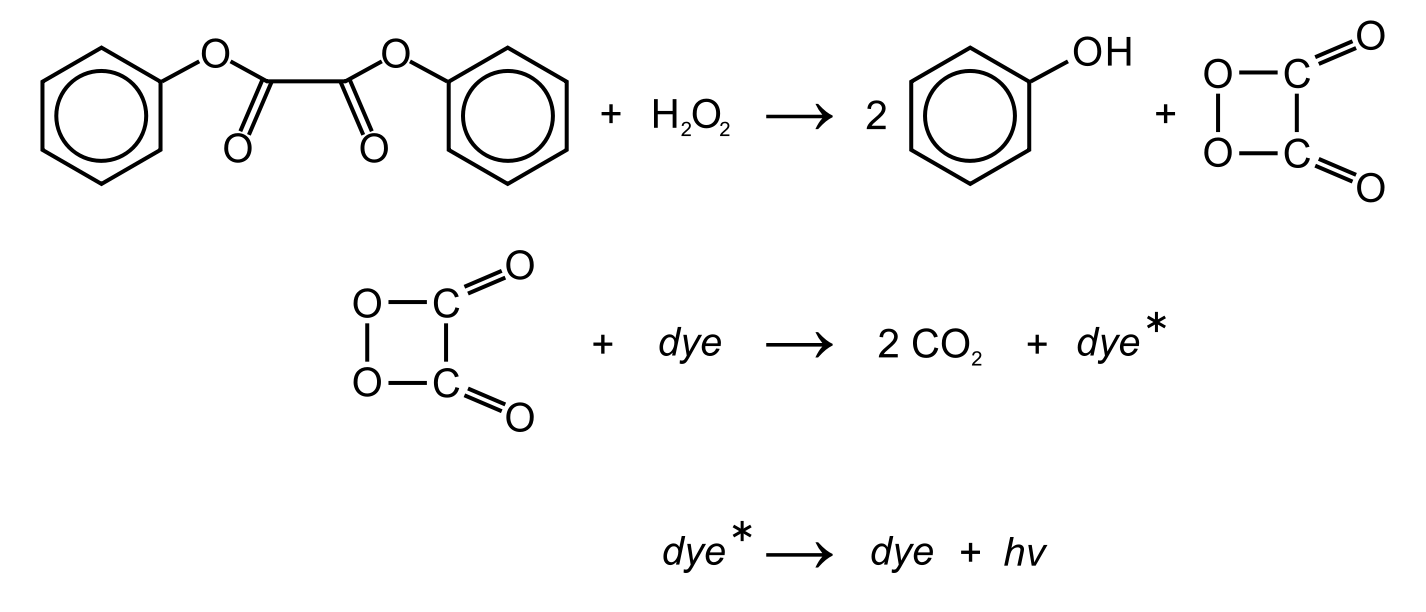
\includegraphics[scale=0.2]{./section/sasakiLIVE/figures/chemical.png}
\caption{シュウ酸ジフェニルと過酸化水素水の反応式}
\label{syu-san}
\end{figure}

\item[(2)ペンライト]\mbox{}\\
電気で光る棒。(非言語大学物理学部の総力を結集してもなお原理は明らかになっていない。CERUNは責任を取り解散した。)

\end{description}

%----------------------------%
\subsubsection{購入}
%----------------------------%

\noindent「あった方が盛り上がる」\\「いや恥ずかしい」\\「高いのでは」\\「奢ってくれるなら買う」\\「自分で買え」\\「奢ってくれるなら買う」\\「奢ってくれるなら買う」\\サイリウムの必要性について我々は激論を交わした。喧々諤々の議論も虚しく、対立構造の崩れぬままサイリウムを買うために一旦会場を離れることとなった。\\
果たしてこの店にサイリウムはあるのか。サイリウムは何のジャンルの商品になるのか。不安を抱きつつ店内を進んだ我々を待っていたのは数百種類はあろうかという莫大な数のサイリウムであった。今回の目的は大魔神の応援であるため、自然と大魔神カラーであるオレンジを選ぶ流れとなった。なお、筆者はある理由により紫を選択したがここでは詳述を避けることとする。\\
ごく自然な流れとしてここでの支払いはアツム氏に一任されることとなり、前述の議論は円満に解決したと言えるだろう。

%----------------------------%
\subsection{俺は地蔵}
%----------------------------%

再びライブ会場に話を戻す。我々が帰還したとき、会場入り口の階段には先ほどまで存在していなかった者どもの群れが発生していた。彼らの存在に恐れ慄いた我々であるが、これより待ち受けるのは大魔神との対決である。尻込みするわけにはいかない。列の最後尾に並び先ほど購入したサイリウムに電池を投入し、開場の時を待った。\\
会場では何故かカレーが販売されていた。夏祭りなどでよく目にするようなビジュアルのカレーである。味も当然、普通のカレーであった。しかし一体なぜライブ中にカレーを食べることができるのか。調査隊は大いに悩まされることとなる。しかしライブを前にしたアツム氏のある発言をきっかけとして、非言語大学文化人類学研究科名誉特任教授Mによってその謎は解明されることとなる。\\
\\
{\Large「俺は地蔵やから」\\}
\\

%----------------------------%
\subsubsection{地蔵}
%----------------------------%

ライブにおける地蔵とは、アイドルの歌や踊り、観客の盛り上がりに反し、定位置で微動だにせず(主に腕を組んで)無言のまま舞台を見つめる者を指す。\\
しかし本来地蔵とは国内の道路にも度々見られる、いわゆる「お地蔵様」に代表されるような仏教的存在であり、その由来は古代インドの伝説上の王にまで遡ることができる。\\
インド?今インドと言ったか?然り。インドである。皆さんはインドと聞いてまず何を思い浮かべるであろうか。ここでは敢えてインド映画を例に挙げよう。インド映画は下の画像に示すように愉快な歌と踊りが特徴である。

\begin{figure}[H]
\centering
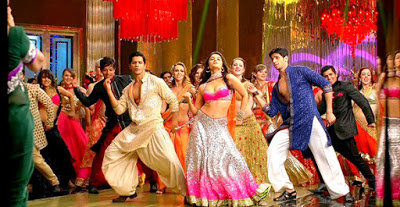
\includegraphics[scale=0.8]{./section/sasakiLIVE/figures/indo.jpg}
\caption{インド映画はとてもよく踊る}
\label{indo}
\end{figure}

愉快な歌と踊りと言えば、アイドルのライブはまさにそれである。ここに$ライブ=インド$の図式が成立した。ライブがインドである以上、そこに地蔵が存在し、インドの国民食であるカレーが供される事は極めて自然な流れだったのである。

\newpage
\clearpage
